\chapter{Experimentos numéricos}
\label{cap:resultados}

Este capítulo contrasta los \crefrange{cap:estructura}{cap:metodos} con
\datoNMetodos{} métodos sobre \datoNEscenarios{} escenarios del motor estudiado.

\section{Diseño experimental}
\subsection{Los escenarios}
Se distinguen \datoNSinteticos{} escenarios sintéticos, \datoNReales{}
cotizaciones RV y \datoNRealesRP{} registros adicionales que incluyen datos de RP.

\paragraph{Escenarios sintéticos.}
Se seleccionan combinaciones de perfiles demográficos y regiones objetivo;
los nueve casos no constituyen el producto cartesiano de todos los perfiles
con todas las regiones. Se incluyen causantes de distinta edad, sexo y
condición de invalidez, con y sin beneficiarios.
\begin{center}
\small
\begin{tabular}{@{}llp{7.2cm}@{}}
\toprule
\textbf{Código} & \textbf{Objetivo} & \textbf{Región estructural} \\
\midrule
\texttt{R2} & $1{,}037\,S_0$ & racimo I: piso del salario mínimo \\
\texttt{R3} & $2{,}414\,S_0$ & tramo afín comercial \\
\texttt{R4} & $5{,}236\,S_0$ & racimo II: activación del auxilio funerario \\
\texttt{R5} & $10{,}372\,S_0$ & racimo III: saturación del auxilio funerario \\
\bottomrule
\end{tabular}
\end{center}
Para cada caso se fija una mesada objetivo y se toma
$\KA=\VP(M_{\mathrm{objetivo}})$. La solución es conocida por construcción,
hasta el redondeo de la evaluación del capital.
\begin{remark}[Elección de los objetivos]
Los objetivos se construyen a partir de constantes irracionales, representadas
en punto flotante. Esto reduce la coincidencia deliberada con los puntos
medios del encaje (\cref{rem:sesgo-diadico}); no elimina el redondeo ni
prueba ausencia de sesgo para toda implementación.
\end{remark}

\paragraph{Cotizaciones reales.}
Los capitales proceden de los archivos de cotización. Las referencias
numéricas obtenidas con Brent a tolerancia estricta se contrastan con una
implementación independiente de SciPy. Se reporta diferencia respecto de
una referencia numérica, no de una solución exacta conocida. La concordancia
con las mesadas de la compañía se analiza aparte en la \cref{sec:validacion}.
Los siete registros adicionales se valoran en este banco con la función
RV: su procedencia no significa que los \datoNMetodos{} métodos se hayan
comparado sobre las recursiones anuales completas de RP.
La financiación exactamente mínima y la insuficiencia se estudian mediante
el \cref{thm:existencia} y comprobaciones específicas; no son casos con
raíz interior incluidos en los porcentajes ordinarios de éxito.

\subsection{Protocolo}
\begin{itemize}[leftmargin=*,nosep]
\item Encaje $[S_0,25S_0]$. El extremo superior es una decisión de búsqueda,
      no un límite contractual general.
\item Arranque abierto: punto medio; secante: extremos; Müller: extremos y punto medio.
\item Tolerancias $\varepsilon_f=\datoEpsilonProd$ peso de capital y
      $\varepsilon_x=10^{-8}$ pesos de mesada, según \cref{eq:parada}.
      El paso pequeño no certifica éxito por sí solo.
\item Diferencias centradas con $h=1$ peso de mesada.
\item Costo: llamadas efectivas al motor, incluidas derivadas y preparación,
      con memoria independiente por método y ejecución.
\end{itemize}
Newton analítico y semisuave calculan conjuntamente valor y derivadas por punto.
Punto fijo, Aitken y Steffensen escalado incluyen la derivada inicial que prepara
la relajación. No se comparte memoria entre métodos ni repeticiones.
Se realizan tres repeticiones de producción; el tiempo por caso es su mediana,
y los promedios por método se calculan después sobre los casos.
Una batería adicional utiliza $\varepsilon_f=10^{-6}$ y $\varepsilon_x=10^{-10}$.
Los tiempos describen el entorno registrado y no garantizan rendimiento en otra máquina.

\section{Resultados globales}
\begin{table}[H]
\centering
\caption[Resultados globales de la comparación]{Comparación sobre
\datoNEscenarios{} escenarios, ordenada por llamadas al motor. «Éxito» indica
cumplimiento del criterio certificado; «Ev.» incluye valor, derivadas y preparación.
El error es la mediana de las diferencias absolutas de mesada respecto de la
referencia. El costo de una ejecución fallida no representa el de una solución.}
\label{tab:resultados-globales}
\small
\begin{tabular}{@{}llrrrrr@{}}
\toprule
\textbf{Método} & \textbf{Familia} & \textbf{Éxito} & \textbf{Ev.\ media} & \textbf{Ev.\ máx.} & \textbf{Iter.} & \textbf{Error mediano} \\
\midrule
Steffensen & abierto & 0\% & 3{,}00 & 3 & 1{,}00 & $1{,}8\cdot10^{6}$ \\
Newton (analítico) & abierto & 100\% & 3{,}08 & 5 & 2{,}08 & $4{,}7\cdot10^{-10}$ \\
Newton semisuave & no suave & 100\% & 3{,}08 & 5 & 2{,}08 & $4{,}7\cdot10^{-10}$ \\
Punto fijo relajado & abierto & 100\% & 3{,}48 & 9 & 2{,}48 & $9{,}3\cdot10^{-10}$ \\
Aitken--Steffensen & abierto & 100\% & 4{,}32 & 5 & 1{,}84 & $0$ \\
Secante & abierto & 100\% & 5{,}08 & 8 & 4{,}08 & $4{,}7\cdot10^{-10}$ \\
Anderson--Björck & encaje & 100\% & 5{,}08 & 8 & 3{,}08 & $3{,}7\cdot10^{-6}$ \\
Pegasus & encaje & 100\% & 5{,}08 & 8 & 3{,}08 & $6{,}6\cdot10^{-6}$ \\
Steffensen escalado & abierto & 100\% & 5{,}24 & 11 & 2{,}12 & $9{,}3\cdot10^{-10}$ \\
Brent & encaje & 100\% & 5{,}28 & 9 & 3{,}28 & $0$ \\
Newton salvaguardado & no suave & 100\% & 5{,}52 & 11 & 2{,}52 & $4{,}7\cdot10^{-10}$ \\
Illinois & encaje & 100\% & 5{,}80 & 9 & 3{,}80 & $4{,}7\cdot10^{-10}$ \\
Regula falsi & encaje & 100\% & 5{,}80 & 11 & 3{,}80 & $3{,}9\cdot10^{-6}$ \\
Müller & abierto & 100\% & 6{,}08 & 9 & 5{,}08 & $1{,}1\cdot10^{-5}$ \\
Newton (dif.\ finitas) & abierto & 100\% & 7{,}60 & 13 & 2{,}20 & $2{,}3\cdot10^{-6}$ \\
Ridders & encaje & 100\% & 9{,}84 & 20 & 3{,}92 & $4{,}7\cdot10^{-10}$ \\
Halley & abierto & 100\% & 10{,}16 & 17 & 3{,}08 & $8{,}4\cdot10^{-6}$ \\
ITP & encaje & 100\% & 29{,}64 & 30 & 27{,}64 & $1{,}1\cdot10^{-3}$ \\
Bisección & encaje & 100\% & 33{,}40 & 35 & 31{,}40 & $1{,}6\cdot10^{-3}$ \\
\bottomrule
\end{tabular}
\end{table}
Newton analítico y semisuave requieren $\datoEvNAN$ llamadas medias.
Con la derivada lateral derecha seleccionada, sus iteraciones coinciden en
esta muestra. Bisección requiere $\datoEvBis$ y Newton con diferencias
finitas, $\datoEvNFD$. La razón de llamadas entre bisección y Newton analítico
es $\datoAceleracionNewton$; la reducción frente a diferencias finitas es
$\datoAhorroDerivada\%$. Estas cifras corresponden al cálculo conjunto verificado;
una implementación con dos llamadas separadas debe contabilizar ambas.
Secante requiere $\datoEvSec$ llamadas y punto fijo, $\datoEvPF$, incluida
la preparación. Halley emplea $\datoEvHal$, sin ventaja frente a Newton en
estos casos. Steffensen sin escalado falla en la batería con los recortes y
la escala empleados (\cref{crit:steffensen}).
\begin{figure}[H]
\centering
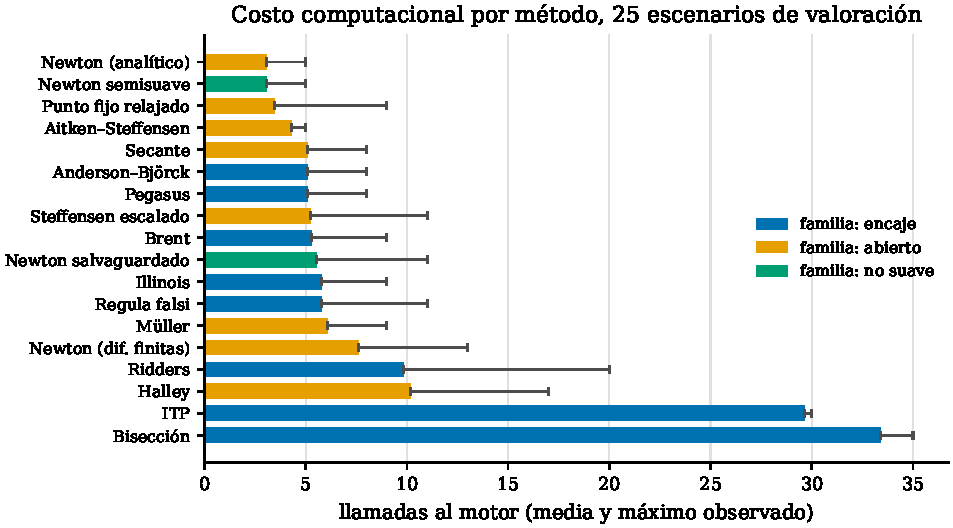
\includegraphics[width=.92\textwidth]{figuras/fig_barras_evaluaciones}
\caption[Costo computacional por método]{Llamadas al motor: media y segmento
hasta el máximo observado. El máximo describe la muestra y no constituye
una cota para una cartera arbitraria.}
\label{fig:barras}
\end{figure}

\section{Alcance de la estimación del orden}
\begin{figure}[H]
\centering
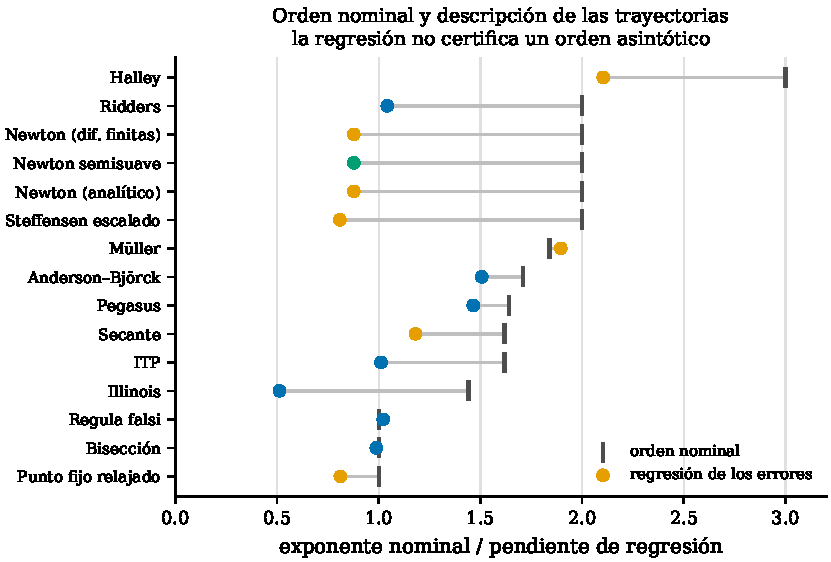
\includegraphics[width=.72\textwidth]{figuras/fig_orden_empirico}
\caption[Orden nominal y estimación por regresión]{Orden nominal y pendiente
estimada por regresión cuando hay suficientes errores útiles. Se omiten los
casos sin estimación o sin orden nominal fijo. Los valores no certifican
por sí solos el orden asintótico.}
\label{fig:orden}
\end{figure}
El orden clásico requiere regularidad y un régimen asintótico. Al cruzar
quiebres pueden faltar esas hipótesis; al alcanzar un tramo afín puede ocurrir
terminación exacta en aritmética ideal. En el segundo caso quedan muy pocos
errores antes del redondeo y el orden no es estimable de forma fiable.
Una regresión sobre iteraciones transitorias no demuestra pérdida del orden
teórico. Se comparan principalmente éxito, residuo, llamadas y tiempo.

\section{Resultados por región estructural}
\label{sec:res-por-region}
\begin{table}[H]
\centering
\caption[Costo por región estructural]{Llamadas medias al motor por región
que contiene la raíz de los escenarios sintéticos.}
\label{tab:por-region}
\small
\begin{tabular}{@{}lrrrr@{}}
\toprule
\textbf{Método} & \textbf{R2 (racimo I)} & \textbf{R3 (afín)} & \textbf{R4 (racimo II)} & \textbf{R5 (racimo III)} \\
\midrule
Bisección & 33{,}0 & 34{,}0 & 34{,}0 & 33{,}0 \\
Brent & 8{,}5 & 5{,}0 & 5{,}0 & 5{,}0 \\
Illinois & 9{,}0 & 6{,}0 & 5{,}0 & 5{,}0 \\
Secante & 8{,}0 & 5{,}0 & 5{,}0 & 5{,}0 \\
Newton (dif.\ finitas) & 13{,}0 & 7{,}0 & 10{,}0 & 7{,}0 \\
Newton (analítico) & 5{,}0 & 3{,}0 & 4{,}0 & 3{,}0 \\
Newton salvaguardado & 10{,}5 & 5{,}0 & 8{,}0 & 5{,}0 \\
Punto fijo relajado & 8{,}5 & 3{,}0 & 5{,}0 & 4{,}0 \\
Halley & 13{,}0 & 10{,}0 & 10{,}0 & 7{,}0 \\
\bottomrule
\end{tabular}
\end{table}
En R3, el paso de Newton obtiene la raíz cuando selecciona la pendiente del
tramo que la contiene (\cref{cor:un-paso}); el resultado no limita a un paso
los arranques exteriores. En R2 la pendiente próxima al mínimo es menor y
cambia al activarse nuevos periodos. En R4 y R5 el cambio del auxilio es pequeño
para las bases examinadas, aunque afecta las garantías basadas en convexidad.
\begin{figure}[H]
\centering
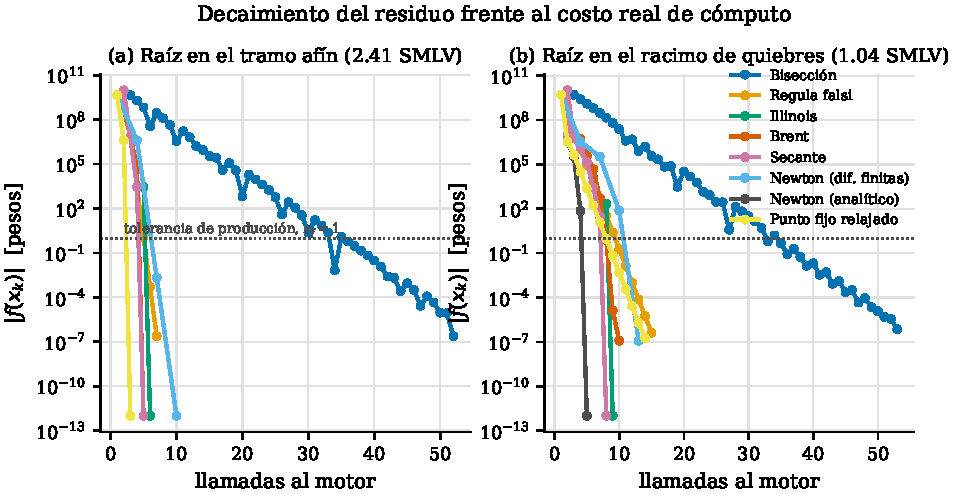
\includegraphics[width=\textwidth]{figuras/fig_convergencia_residuos}
\caption[Decaimiento del residuo]{Residuo de valoración frente a llamadas
acumuladas al motor, en escala logarítmica. La línea horizontal indica un
peso de capital; los paneles corresponden al tramo afín y al racimo I.}
\label{fig:residuos}
\end{figure}
\begin{figure}[H]
\centering
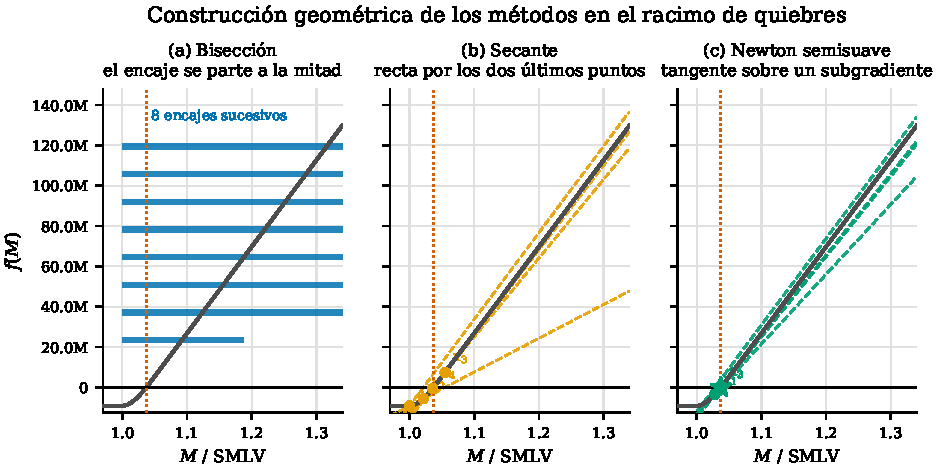
\includegraphics[width=\textwidth]{figuras/fig_trayectorias}
\caption[Construcción geométrica de los métodos]{Construcción de bisección,
secante y Newton semisuave cerca del racimo I. La ampliación muestra cambios
de pendiente y no sustituye las hipótesis de los teoremas.}
\label{fig:trayectorias}
\end{figure}

\section{Robustez frente al punto inicial}
\label{sec:robustez-empirica}
\begin{figure}[H]
\centering
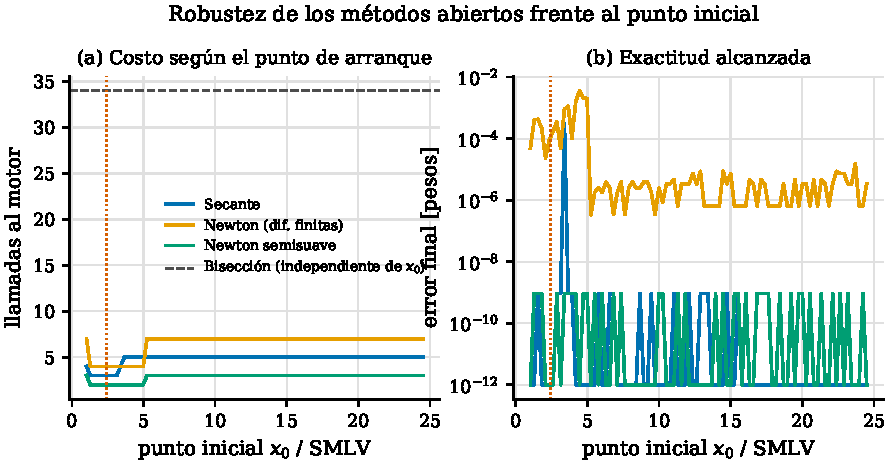
\includegraphics[width=\textwidth]{figuras/fig_robustez_inicial}
\caption[Robustez frente al punto inicial]{Costo y error final para A-R3,
en una malla de 90 arranques entre $1{,}02S_0$ y $24{,}5S_0$.
Cada ejecución dispone de memoria propia y se comprueba el residuo.}
\label{fig:robustez}
\end{figure}
El barrido describe un escenario y una malla finita. Los métodos con encaje,
incluidos la variante salvaguardada y Brent, parten del intervalo inicial y no
de $x_0$; por eso solo la bisección figura en el barrido, como referencia.
La convergencia monótona
del \cref{thm:terminacion-finita}(ii) requiere convexidad en el intervalo
recorrido y arranque a la derecha. La variante salvaguardada dispone de la
garantía del \cref{thm:salvaguardado}; Brent y otros métodos con encaje también
ofrecen garantías bajo sus condiciones. El barrido no demuestra robustez global
de los métodos abiertos para cualquier póliza.

\section{Costo frente a precisión exigida}
\begin{figure}[H]
\centering
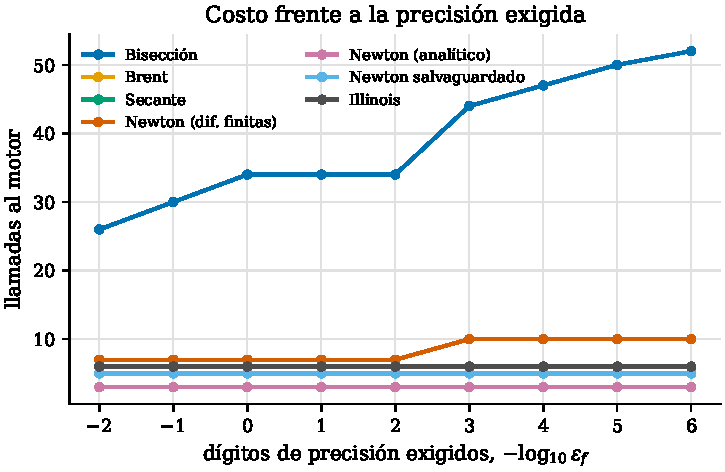
\includegraphics[width=.78\textwidth]{figuras/fig_costo_tolerancia}
\caption[Costo frente a precisión]{Llamadas al motor frente a tolerancia de
residuo en A-R3. El costo casi constante de algunos métodos corresponde a
este escenario y al rango de tolerancias representado.}
\label{fig:costo-tolerancia}
\end{figure}
La cota de bisección aumenta aproximadamente $\log_2(10)$ pasos por dígito
decimal adicional de exactitud en la variable. En un tramo afín, Newton con
pendiente exacta puede alcanzar el redondeo sin iteraciones adicionales al
endurecer la tolerancia. Una tolerancia inferior al residuo alcanzable en punto
flotante no implica convergencia ni exactitud adicional.

\section{Contraste sobre cotizaciones reales}
Las soluciones de los dos conjuntos reales se sitúan entre $\datoMultMin$ y
$\datoMultMax$ salarios mínimos, con media $\datoMultMedia$. En esta muestra
quedan en el tramo afín $[\datoAnchoRacimo,5]S_0$. Esto explica la utilidad de
la pendiente exacta; no prueba que toda la cartera o todo el mercado tenga
esa propiedad ni valida las bases actuariales. El contraste de la
\cref{sec:validacion} requiere conciliar datos, hipótesis y recargos.

\section{Hallazgos sobre la implementación de producción}
\label{sec:hallazgos-codigo}
Se distingue la corrección del banco de su adopción en todos los flujos de producción.
\begin{table}[H]
\centering
\caption[Recomendaciones sobre la implementación]{Correcciones y recomendaciones.
La verificación del catálogo no certifica todos los recorridos de la aplicación.}
\label{tab:hallazgos}
\small
\begin{tabular}{@{}>{\raggedright\arraybackslash}p{.55cm}>{\raggedright\arraybackslash}p{4.1cm}>{\raggedright\arraybackslash}p{5.2cm}>{\raggedright\arraybackslash}p{3.1cm}@{}}
\toprule
& \textbf{Acción} & \textbf{Fundamento} & \textbf{Estado} \\
\midrule
R1 & Distinguir insuficiencia de fallo numérico. & $\KA<\VP(S_0)$ identifica
insuficiencia; el fracaso del método no la demuestra. & Comprobado en sensibilidad;
integración general pendiente. \\
\midrule
R2 & Corregir la derivada en $M=S_0$. & \cref{prop:continuidad-rama}: la rama
altera la fórmula de la derivada aunque conserve el valor. & Implementado en el motor. \\
\midrule
R3 & Certificar el error y declarar sus unidades. & $|x-M^*|\le |f(x)|/m$
requiere cota inferior válida; el ancho del encaje ofrece otro certificado. &
Criterio corregido en el banco. \\
\midrule
R4 & Elegir la tolerancia anual de RP según horizonte. & \cref{cor:tolerancia-rp}:
intervienen el estado acoplado, rendimientos y errores locales. & Cota formulada;
calibración operativa pendiente. \\
\midrule
--- & Calcular conjuntamente valor y derivada. & Una llamada por punto;
ahorro observado de $\datoAhorroDerivada\%$ frente a diferencias finitas. &
Implementado y contado en el banco. \\
\bottomrule
\end{tabular}
\end{table}

\section{Recomendación}
\begin{aporte}
Para el modelo estudiado, cuando se dispone de la derivada analítica, se recomienda
Newton semisuave con salvaguarda periódica (\cref{alg:newton-salvaguardado}).
Combina la reducción cuantitativa del encaje con la terminación local afín a
trozos. En la batería completa emplea $\datoEvNSG$ llamadas medias, frente a
$\datoEvBis$ de bisección, $\datoEvSec$ de secante y $\datoEvBre$ de Brent.

La comparación con Brent depende de la región de la raíz. En las cotizaciones
reales, situadas en el tramo afín, el salvaguardado requiere $4{,}78$ y
$4{,}71$ llamadas medias en los dos conjuntos, frente a $5{,}00$ de Brent; las
dos llamadas adicionales respecto de Newton semisuave sin salvaguarda
corresponden a la evaluación de los extremos del encaje. En los escenarios
sintéticos, que sitúan deliberadamente raíces en los racimos de quiebres,
requiere $6{,}89$ frente a $5{,}78$ de Brent (\cref{tab:por-region}).

La preferencia por el salvaguardado no descansa, por tanto, en un menor costo
en todos los casos. Se apoya en que aprovecha la pendiente exacta para obtener
la raíz por inversión del tramo que la contiene, en que su paso tiene una
lectura actuarial directa (\cref{thm:subdiferencial}) y en la cota global del
\cref{thm:salvaguardado}, que no es la misma cota por iteración de la bisección
pura. Cuando no se dispone de derivadas, Brent ofrece una alternativa con encaje
y costo similar. La secante es competitiva en costo, pero su versión abierta
carece de esa garantía global. La elección operativa requiere verificar dominio,
bases actuariales y certificados de salida.
\end{aporte}
